\documentclass[]{article}

%%use packages%%
\usepackage[utf8]{inputenc}
\usepackage [english]{babel}
\usepackage [autostyle, english = american]{csquotes}
\usepackage[export]{adjustbox}
\usepackage{lipsum}
\usepackage{titlesec}
\usepackage{lmodern}
\usepackage{titling}
\usepackage{amssymb,amsmath}
\usepackage{ifxetex,ifluatex}
\usepackage{multicol}
\usepackage[a4paper, total={6in, 9in}]{geometry} %margin
\usepackage{fixltx2e} % provides \textsubscript
\usepackage{listings}
\usepackage{color}
\usepackage{caption}
\usepackage[]{microtype}
\usepackage{graphicx}
\usepackage{wrapfig}
\graphicspath{ {images/}}

\setlength{\columnsep}{0.7cm}

% use microtype if available
\IfFileExists{microtype.sty}{%
	
	\UseMicrotypeSet[protrusion]{basicmath} % disable protrusion for tt fonts
}{}
\PassOptionsToPackage{hyphens}{url} % url is loaded by hyperref
\usepackage{xcolor}
\usepackage[colorlinks = true,
linkcolor = blue,
urlcolor  = blue,
citecolor = blue,
anchorcolor = blue]{hyperref}
\hypersetup{linkcolor=black}
\newcommand{\MYhref}[3][blue]{\href{#2}{\color{#1}{#3}}}%
\hypersetup{
	pdfborder={0 0 0},
	breaklinks=true}
\urlstyle{same}  % don't use monospace font for urls

\MakeOuterQuote{"}
%define subtitle
\newcommand{\subtitle}[1]{%
	\posttitle{%
		\par\end{center}
	\begin{center}\large#1\end{center}
	\vskip0.5em}%
}

%define indentations & sections spacing
\setlength{\parindent}{4em}
\titlespacing\section{0pt}{12pt plus 4pt minus 2pt}{0pt plus 4pt minus 2pt}

%%%%%%%%%%%%%%%%%%%%%%%%%%%%%%%%%%%%%%%%%%%%%%%%%%%%%%%
\begin{document}

\title{Encrypted Messaging Application with RSA Public-Key Cryptosystems}
\subtitle{Deerfield Academy Advance Computer Science Research}

\author{Yongyang (Neil) Nie}

\date{May, 2017}

\maketitle

\tableofcontents

\vspace{2.0cm}

%%%%%%%%%%%%%%%%%%%%%%%%%%%%%%%%%%%%%%%%%%%%%%%%%%%%%%%

\subsubsection{Abstract}
From online payment to check our email, RSA is the most widely used Public-Key cryptosystems in the world. It takes advantages of the P vs. NP problem (the difficult prime factorizing problem) in order to encrypt data. First discovered by Rivest, Shamir and Adleman in 1977, the algorithm has never been compromised, which is also why RSA is one of the most copied software in the world. In the spring of 2017, I developed an iOS application that uses RSA to send encrypted messages. 

\section{Introduction}
Encryption is a way to conceal a message which can only be opened by using a unique key. Encryption is the about reversing the encryption process with that unique key. Imagine that Bob wants to send Alice an encrypted message, somehow, they have to share the same key to decrypt the message. However, exchanging a synchronized key is very difficult. Prior to the 1970s, encryption relied on algorithms such as the Diffie–Hellman key exchange \footnote{https://en.wikipedia.org/wiki/Diffie–Hellman\_key\_exchange}. In 1977, Rivest, Shamir and Adleman discovered RSA, a Public-Key Cryptosystem, which is safer and much more friendly than the traditional methods. \footnote{Please refer to: https://www.khanacademy.org/computing/computer-science/cryptography/modern-crypt/v/} Until today, RSA is till the most widely used encryption scheme in computer science. 

\section{Public-Key Cryptosystems}

Public-Key encryption, also known as asymmetric encryption, is any cryptographic system that uses pairs of keys: public keys which may be disseminated widely, and private keys which are known only to the owner. \footnote{https://en.wikipedia.org/wiki/Public-key\_cryptography} In this system, a user an encrypt a message with receiver's public key, and only the receiver can decrypt with message with his private key. 
\section{RSA Encryption Algorithm}
RSA is an algorithm used by modern computers to encrypt and decrypt messages. It is an asymmetric cryptographic algorithm. Asymmetric means that there are two different keys. This is also called public key cryptography, because one of them can be given to everyone. The other key must be kept private. It is based on the fact that finding the factors of an integer is hard (the factoring problem). RSA stands for Ron Rivest, Adi Shamir and Leonard Adleman, who first publicly described it in 1978. A user of RSA creates and then publishes the product of two large prime numbers, along with an auxiliary value, as their public key. The prime factors must be kept secret. Anyone can use the public key to encrypt a message, but with currently published methods, if the public key is large enough, only someone with knowledge of the prime factors can feasibly decode the message.[1]


\subsection{The Mathematics Behind RSA}

RSA requires a math function that is easy to compute but hard to reverse, except if you have a special key. Multiplication is very easy to compute on modern computers, however, prime factorization \footnote{For more on prime factorization: http://mathworld.wolfram.com/PrimeFactorization.html} is very difficult. In fact, the time complexity for multiplication grows \textit{linearl}  as the number of digits increases; the time complexity for prime factorization grows \textit{exponentially} as the number increase. 

\centerline{ 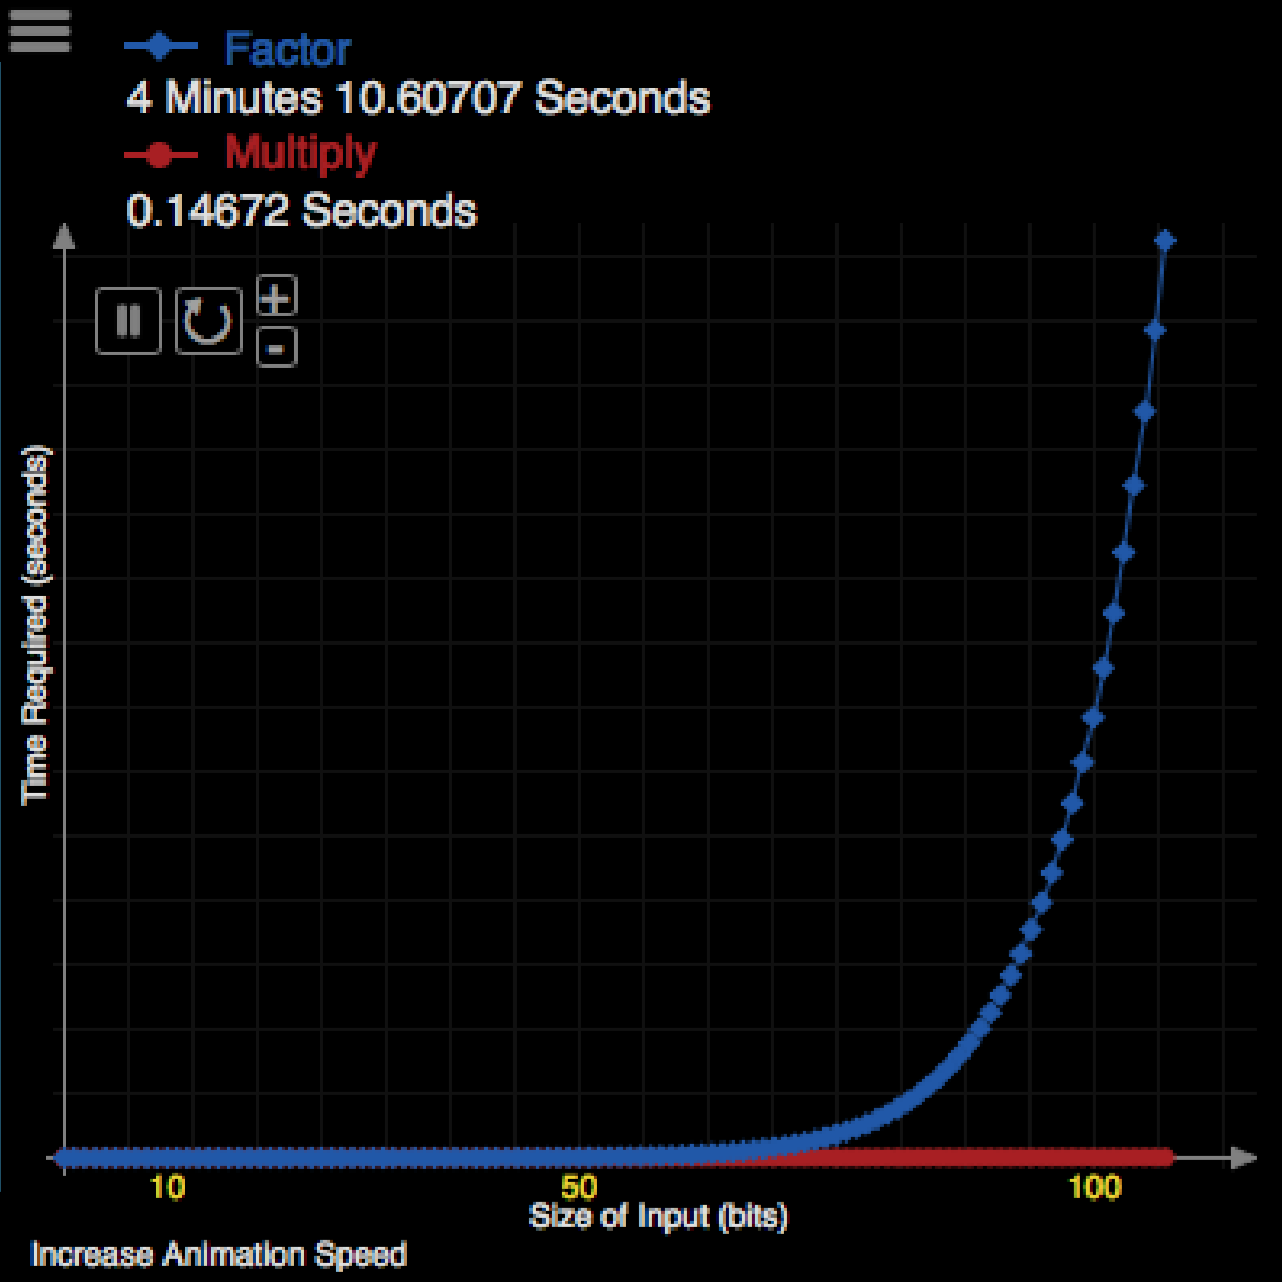
\includegraphics[scale=0.20]{time_complex}} \footnote{From Khan Academy}

The RSA takes advantages of the fact above to create a one-way, trapdoor function. This function allows the user to easy to encrypt a message with a public key, however, can't be decrypted with brute force within a reasonable amount of time. Another user, with the trapdoor (a.k.a the private key) can decrypt the message easily. 

A basic principle behind RSA is the observation that it is practical to find three very large positive integers e, d and n such that with modular exponentiation for all integer m:

\[ (m^{e})^{d}\equiv m{\pmod {n}}\]
and that even knowing e and n or even m it can be extremely difficult to find d.

Additionally, for some operations it is convenient that the order of the two exponentiations can be changed and that this relation also implies:

\[(m^{d})^{e}\equiv m{\pmod {n}}\]
The public key is represented by the integers n and e; and, the private key, by the integer d (although n is also used during the decryption process; so, it might be considered a part of the private key, too). m represents the message.

\subsubsection{Key generation}

The keys for the RSA algorithm are generated the following way:

Choose two distinct prime numbers p and q. For security purposes, the integers p and q should be chosen at random. The size of the primes are typically 1,024 to 4,096 bit. They should be similar in magnitude but differ in length by a few digits to make factoring harder. Prime integers can be efficiently found using a primality test.

\begin{equation}
	n = pq
\end{equation}
n is the modulus for the public key and the private key.

\begin{equation}
	 \phi (n)=(p-1)(q-1)
\end{equation}
Choose an integer e such that \(1 < e < \phi(n)\) and \(gcd(e, \phi(n)) = 1\). Also, i, e and \(\phi(n)\) are coprime.

\begin{equation}
	d \equiv e^{-1} (\mod\phi(n))
\end{equation}
This is more clearly stated as: solve for d given \(d * e \equiv 1 (\mod \phi(n))\).
\begin{equation}
	e \equiv \text{small  prime  number}
\end{equation}
e is released as the public key exponent.

The public key: the modulus n and the public (or encryption) exponent e. 

The private key: the modulus n and the private (or decryption) exponent d, which must be kept secret. p, q, and \(\phi(n)\) must also be kept secret because they can be used to calculate d.

\bigskip

It's important to note that the encryption process has evolved since the first publication of the RSA paper \footnote{The first RSA paper \href{https://goo.gl/UWT0zd}{link}}. Equation 2 changed in PKCS\#1 v2.0 to \( \lambda (n)={\rm {lcm}}(p-1,q-1)\). Also, in equation 4, A popular choice for the public exponents is \(e = 2^{16} + 1 = 65537\). Some applications choose smaller values such as \(e = 3, 5, or 35\)  instead. This is done to make encryption and signature verification faster on small devices like smart cards but small public exponents may lead to greater security risks \footnote{This is reference from Wikipeida: https://simple.wikipedia.org/wiki/RSA\_(algorithm)}.

\subsubsection{Key distribution}
Suppose that Bob wants to send a secret message to Alice. Bob must know Alice's public key to encrypt the message and, Alice must use her private key to decrypt the message. To enable Bob to send his encrypted messages, Alice send her public key (n, e) to Bob. Even if the public key is intercepted, anyone but Alice will not be able to decrypt Bob's secret message. 

\subsubsection{Encryption}
After Bob obtains Alice's public key, he can send a message m to Alice.

To do so, he first turns plain text into an integer m, using a padding \footnote{For more on padding scheme: https://en.wikipedia.org/wiki/Padding\_(cryptography)} and encoding scheme.  The encoding should be easily reversed by the receiver of the message. The padding scheme is useful and secure but not necessary. He then computes the ciphertext c, using Alice's public key e, corresponding to
\[c \equiv m^e \pmod{n} \]
This can be done very quickly on a personal computer or a smartphone, if if the number exceed 500 bits.

\subsubsection{Decryption}
Alice can recover m from c by using her private key exponent d by computing

\[{c^{d}\equiv (m^{e})^{d}\equiv m{\pmod {n}}}\]
Given m, she can recover the original message M by reversing the padding scheme.

\subsection{A Quick Example}\footnote{This example is from Universe of Texas https://www.cs.utexas.edu/~mitra/honors/soln.html}

Choose p = 3 and q = 11 
\[n = p * q = 3 * 11 = 33\]
\[\phi(n) = (p - 1) * (q - 1) = 2 * 10 = 20\]

Choose e such that \(1 < e < \phi(n)\) and e and \(\phi (n)\) are coprime. Let e = 7

Compute a value for d such that \((d * e)\mod  \phi(n) = 1\). One solution is \(d = 3, (3 * 7) \mod 20 = 1\)

Public key is (e, n) = (7, 33)

Private key is (d, n) = (3, 33)

The encryption of m = 2 is \(c = 2^{7} \mod 33 = 29\)

The decryption of c = 29 is \(m = 29^{3} \mod 33 = 2\)

\subsection{Why does it work?}

If you are reading this paper, you probably have heard of the P vs. NP problem. Informally speaking, "it asks whether every problem whose solution can be quickly verified by a computer can also be quickly solved by a computer." 

The term "quickly" means the existence of an algorithm that can solve the problem in polynomial time. The time to complete the task varies as the size of the input varies. Problem can be answer in polynomial time are called "P". For some questions, there is no known way to find an answer quickly. But if the information about the answer is provided, then it's possible to verify the answer quickly. The class of questions for which an answer can be verified in polynomial time is called NP, which stands for "nondeterministic polynomial time."\footnote{Referenced from: https://en.wikipedia.org/wiki/P\_versus\_NP\_problem}.

RSA takes advantages of the P vs. NP problem. It's easy to multiply numbers, but difficult to find the prime factors. It's easy if we are given one of the prime numbers. With those properties in mind, up until the point this paper is written, no one has been able to compromise the algorithms, thanks to the unsolved P vs. NP problem. 

\section{RSA in practical use}

The major part of this project is to use RSA to create an encrypted messaging app. Theoretical RSA is different from implementations. There are many obstetrical and problems to consider. 

\subsection{String Encoding \&  Decoding}

The second challenge is encoding numbers with strings, vice versa. There are many different kinds of encoding scheme used for RSA. They are generally very simple to compute. One popular encoding is to convert a piece of string to a bit array, then convert it into an integer. By using ASCII \footnote{https://en.wikipedia.org/wiki/ASCII}, character can be converted into integers, then join those numbers together to form the message. 

\subsection{Databases and Multiuser Authentication}

The keys and values from the RSA algorithm has to be encoded and stored as a string in a backend, custom built by the developer or via certain backend service. Specifically, I am using Firebase, by Google as my backend. It's a secure and fast real-time database service. The encoding scheme is already mentioned above. Firebase is a real-time database. The app automatically listen to change in the backend. The app simply needs to have an observer for data change in the data base, and all parties in that conversation will be updated. 

The database also stores the public key for each users. Upon installing the application, it will prompt the user to login or register. When a user registers for the first time, the public keys will be randomly generated. The keys are stored locally (hashed and secure), as well as in the backend. Interestingly, the app send the server HTTPS requests, (Hypertext Transfer Protocol Secure) which is an advanced version of RSA. 

\subsection{Working with Prime numbers}

First, handling large prime numbers, around 1024 bits, can be challenging. There are two ways to gain access to those large primes. There are libraries of prime numbers that developers can reference from. However, this can be unsafe, in that hackers might be able to compromise the database information. The more widely used approach is to generate prime numbers. The standard way to generate big prime numbers is to take a preselected random number of the desired length, apply a Fermat test \footnote{More on Fermat Test: https://en.wikipedia.org/wiki/Fermat\_primality\_test} (best with the base 2 as it can be optimized for speed) and then to apply a certain number of Miller-Rabin tests \footnote{More on Miller-Rabin test https://en.wikipedia.org/wiki/Miller–Rabin\_primality\_test} (depending on the length and the allowed error rate like \(2^{-100}\)) to get a number which is very probably a prime number. 

In order to perform RSA securely, some large integer class needs to be implemented. In C, the max size for unsigned long is 20 digits \footnote{Data from C stand library, <limits.h> https://www.tutorialspoint.com/c\_standard\_library/limits\_h.htm}, which is far from what a secure RSA needs. Since my project is developed in Objective-C, I used the LibTomMath \footnote{From: http://www.libtom.net} library and a simple wrapper. 

\section{Conclusion}

In this project, the basics of RSA are introduced. The mathematics behind the algorithm is also explored. With these knowledge, an iOS encrypted messaging application is developed. While developing the app, I encountered many unexpected challenges, from generating prime numbers to encoding strings. 

It's proven that RSA is one of the most secure public key algorithms ever invented. It powers online banking, messaging and protects Internet privacy. There are many other version of RSA and other public key cryptosystems. They are adapted to specific purposes. In the future, I can further explore the beauty and power of cryptosystems. 

\end{document}